\let\negmedspace\undefined
\let\negthickspace\undefined
\documentclass[journal,12pt,onecolumn]{IEEEtran}
\usepackage{cite}
\usepackage{amsmath,amssymb,amsfonts,amsthm}
\usepackage{algorithmic}
\usepackage{graphicx}
\graphicspath{{./figs/}}
\usepackage{textcomp}
\usepackage{xcolor}
\usepackage{txfonts}
\usepackage{listings}
\usepackage{enumitem}
\usepackage{mathtools}
\usepackage{gensymb}
\usepackage{comment}
\usepackage{caption}
\usepackage[breaklinks=true]{hyperref}
\usepackage{tkz-euclide} 
\usepackage{listings}
\usepackage{gvv}                                        
%\def\inputGnumericTable{}                                 
\usepackage[latin1]{inputenc}     
\usepackage{xparse}
\usepackage{color}                                            
\usepackage{array}                                            
\usepackage{longtable}                                       
\usepackage{calc}                                             
\usepackage{multirow}
\usepackage{multicol}
\usepackage{hhline}                                           
\usepackage{ifthen}                                           
\usepackage{lscape}
\usepackage{tabularx}
\usepackage{array}
\usepackage{float}
\newtheorem{theorem}{Theorem}[section]
\newtheorem{problem}{Problem}
\newtheorem{proposition}{Proposition}[section]
\newtheorem{lemma}{Lemma}[section]
\newtheorem{corollary}[theorem]{Corollary}
\newtheorem{example}{Example}[section]
\newtheorem{definition}[problem]{Definition}
\newcommand{\BEQA}{\begin{eqnarray}}
\newcommand{\EEQA}{\end{eqnarray}}
\newcommand{\define}{\stackrel{\triangle}{=}}
\theoremstyle{remark}
\newtheorem{rem}{Remark}



\title{\LARGE \textbf{AE - 2017}}
\author{\Large EE25BTECH11048 - Revanth Siva Kumar.D}
\date{}

\begin{document}

\maketitle
\begin{flushleft}
\begin{enumerate}
\item
Given the vectors 
\begin{align*}
\vec v_{1} &= \hat{i}+3\hat{j}, \\
\vec v_{2} &= 2\hat{i}-4\hat{j}+3\hat{k},
\end{align*}
the vector $\vec v_{3}$ that is perpendicular to both $\vec v_{1}$ and $\vec v_{2}$ is given by:  
\hfill (GATE AE 2017)

\begin{enumerate}
\begin{multicols}{2}
\item $\vec v_{3}=\vec v_{1}-\big(\vec v_{1}\cdot \vec v_{2}\big)\,\dfrac{\vec v_{2}}{\abs{\vec v_{2}}^{2}}$
\item $\vec v_{3}=\hat{k}$
\item $\vec v_{3}=\vec v_{2}-\big(\vec v_{1}\cdot \vec v_{2}\big)\,\dfrac{\vec v_{1}}{\abs{\vec v_{1}}^{2}}$
\item $\vec v_{3}=\dfrac{\vec v_{1}}{\abs{\vec v_{1}}}\times\dfrac{\vec v_{2}}{\abs{\vec v_{2}}}$
\end{multicols}
\end{enumerate}

\item
The value of the integral
\begin{align*}
I=\oint_{C}\big((x-y)\,dx+x^{2}\,dy\big), \qquad
C:\ 0\le x\le 2,\ 0\le y\le 2,
\end{align*}
is \underline{\hspace{2cm}}  
\hfill (GATE AE 2017)

\item
Let $\vec v(t)$ be a unit vector that is a function of the parameter $t$. Then
\begin{align*}
\vec v\cdot \frac{d\vec v}{dt} &= \underline{\hspace{2cm}}
\end{align*}
\hfill (GATE AE 2017)

\item
The eigenvalues $\lambda_n$ and eigenfunctions $u_n(x)$ of the Sturm-Liouville problem
\begin{align*}
\frac{d^{2}y}{dx^{2}}+k^{2}\lambda\,y&=0,\qquad 0<x<1,\\
y(0)&=0,\qquad y(1)=0
\end{align*}
are given by:  
\hfill (GATE AE 2017)

\begin{enumerate}
\item $\lambda_n=n^{2}\pi^{2},\quad u_n(x)=\sin(\lambda_n x),\quad n=0,\pm1,\pm2,\dots$
\item $\lambda_n=\dfrac{n^{2}\pi^{2}}{k^{2}},\quad u_n(x)=\sin(kn\pi x),\quad n=0,\pm1,\pm2,\dots$
\item $\lambda_n=\dfrac{n^{2}\pi^{2}}{k^{2}},\quad u_n(x)=\sin(n\pi x),\quad n=0,\pm1,\pm2,\dots$
\item $\lambda_n=n^{2}\pi^{2},\quad u_n(x)=\sin(n\pi x),\quad n=0,\pm1,\pm2,\dots$
\end{enumerate}

\item
3-point Gaussian integration formula is given by:
\begin{align*}
\int_{-1}^{1} f(x)\, dx \;\approx\; \sum_{j=1}^{3} A_j f(x_j) 
\quad \text{with} \quad 
x_1=0,\; x_2=-x_3=-\sqrt{\tfrac{3}{5}}, \quad 
A_1=\tfrac{8}{9},\; A_2=A_3=\tfrac{5}{9}.
\end{align*}
This formula exactly integrates \hfill (GATE AE 2017)

\begin{enumerate}
\begin{multicols}{2}
\item $f(x)=5-x^7$
\item $f(x)=2+3x+6x^4$
\item $f(x)=13+6x^3+x^6$
\item $f(x)=e^{-x^2}$
\end{multicols}
\end{enumerate}

\item
Which one of the following statements is NOT true?  
\hfill (GATE AE 2017)

\begin{enumerate}
\item The pitching moment of any airfoil at any angle of attack is always zero at the center of pressure
\item The pitching moment of any airfoil at any angle of attack is always zero at the aerodynamic center
\item The center of pressure and aerodynamic center coincide for a symmetric airfoil
\item The pitching moment about the aerodynamic center, for any airfoil, does not vary with angle of attack
\end{enumerate}

\item
Which one of the following statements is NOT true?  
\hfill (GATE AE 2017)

\begin{enumerate}
\item Compared to a laminar boundary layer, a turbulent boundary layer is more desirable on a wing operating at large angle of attack
\item The skin friction drag for a turbulent boundary layer is larger than that for a laminar boundary layer
\item The location of transition from laminar to turbulent boundary layer depends only on the operating Reynolds number
\item A separated flow does not necessarily lead to a turbulent boundary layer
\end{enumerate}

\item
A De Laval nozzle is to be designed for an exit Mach number of 1.5. The reservoir conditions are given as $P_0=1$ atm (gage), $T_0=20^\circ$C, $\gamma=1.4$. Assuming shock free flow in the nozzle, the exit absolute pressure (in atm) is \underline{\hspace{2cm}} (in three decimal places).  
\hfill (GATE AE 2017)
\item Consider a steady one dimensional flow of a perfect gas with heat transfer in a duct. The T-s diagram (shown below) shows both the static and the stagnation conditions at two locations, A and B, in the duct. $A_t$ and $B_t$ denote stagnation conditions for states A and B, respectively. It is known that 
\begin{align*}
(\Delta T)_A = (\Delta T)_B
\end{align*}
$M_A$ and $M_B$ are the Mach numbers of the flow at locations A and B. \hfill (GATE AE 2017)
\begin{figure}[H]
    \centering
    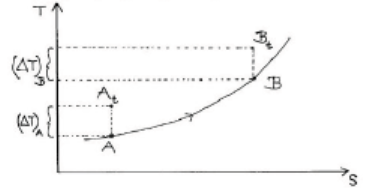
\includegraphics[width=0.5\columnwidth]{figs/9.png}
    \caption{}
    \label{fig:placeholder}
\end{figure}
\begin{enumerate}
\item Flow is subsonic and $M_A < M_B$
\item Flow is supersonic and $M_A > M_B$
\item Flow is subsonic and $M_A > M_B$
\item Flow is supersonic and $M_A < M_B$
\end{enumerate}


\item To ensure only the longitudinal static stability (and not the condition for equilibrium) of a low speed aircraft, the aircraft components must be designed to satisfy which one of the following conditions: \hfill (GATE AE 2017)

\begin{enumerate}
\item $\dfrac{\partial C_m}{\partial \alpha} < 0 \quad \text{and} \quad C_{m0} > 0$
\item $\dfrac{\partial C_m}{\partial \alpha} \leq 0$
\item $\dfrac{\partial C_L}{\partial \alpha} < 0 \quad \text{and} \quad C_{m0} < 0$
\item $\dfrac{\partial C_m}{\partial C_L} = 0.0$
\end{enumerate}


\item Which of the following statement(s) is/are true about the shear centre of a cross-section:  
P: It is that point in the cross-section through which shear loads produce no twisting.  
Q: This point is also the centre of twist of sections subjected to pure torsion.  
R: The normal stress at this point is always zero.  
\hfill (GATE AE 2017)

\begin{enumerate}
\item P, Q and R
\item P only
\item P and Q only
\item P and R only
\end{enumerate}

\item Let $\bar{N}_m$ and $\bar{N}_0$ be respectively the non-dimensional locations of the stick-fixed maneuver point and stick-fixed neutral point of a low speed conventional aircraft. These distances are measured with respect to the nose of the fuselage. The numerical value of $\bar{N}_m - \bar{N}_0$ 
\hfill (GATE AE 2017)

\begin{multicols}{2}
\begin{enumerate}
\item will always be negative
\item will always be positive
\item will always be zero
\item can have any value depending on the location of the center of gravity of the aircraft
\end{enumerate}
\end{multicols}

\item The phenomenon of rudder lock in conventional low speed aircraft is primarily due to 

\hfill (GATE AE 2017)

\begin{enumerate}
\item large value of directional derivative, $C_{n\beta}$
\item the sidewash due to fuselage on the vertical stabilizer
\item the tendency of rudder to float rapidly at high angles of side-slip
\item the sidewash due to wing on the vertical stabilizer
\end{enumerate}

\item The period of revolution of earth about the sun is 365.256 days, approximately. The semi-major axis of the earth's orbit is close to $1.4953 \times 10^{11}$ m. The semi-major axis of the orbit of Mars is $2.2783 \times 10^{11}$ m. The period of revolution of Mars, about the sun, is \underline{\hspace{2cm}} Earth days (in three decimal place).  
\hfill (GATE AE 2017)

\item Consider a system consisting of certain amount of perfect gas enclosed in a cylinder fitted with a frictionless piston. This system can undergo following processes:  
(i) Expansion with finite pressure difference with the surrounding.  
(ii) Compression with infinitesimal pressure difference with the surrounding.  
(iii) Heat transfer with finite temperature difference with the reservoir.  
(iv) Heat transfer with infinitesimal temperature difference with the reservoir.  

Out of these which processes are reversible?
\hfill (GATE AE 2017)

\begin{multicols}{2}
\begin{enumerate}
\item (i) and (iii)
\item (ii) and (iv)
\item (ii) and (iii)
\item (i) and (iv)
\end{enumerate}
\end{multicols}

\item Among the following engines, which one is expected to have the maximum Specific Impulse? 
\hfill (GATE AE 2017)

\begin{multicols}{2}
\begin{enumerate}
\item Cryogenic Rocket
\item Solid Propellant Rocket
\item Liquid Propellant Rocket
\item SCRAM Jet
\end{enumerate}
\end{multicols}

\item The maximum gas flow rate that can be handled by a multistage axial compressor at a given rotational speed is dictated by 
\hfill (GATE AE 2017)

\begin{multicols}{2}
\begin{enumerate}
\item Compressor Surge
\item Rotating Stall
\item Choking
\item Optimum Design Pressure Ratio
\end{enumerate}
\end{multicols}

\item For a turbine stage, which one of the following losses occurs due to the turning of the wall boundary layer through an angle due to curved surface? 
\hfill (GATE AE 2017)

\begin{multicols}{2}
\begin{enumerate}
\item Profile loss
\item Annulus loss
\item Tip clearance loss
\item Secondary flow loss
\end{enumerate}
\end{multicols}

\item In the vane-less space between the impeller and the diffuser vanes in a Centrifugal Compressor, the angular momentum varies in the following manner in the radial direction  

\hfill (GATE AE 2017)

\begin{multicols}{2}
\begin{enumerate}
\item Increases
\item Remains constant
\item Decreases
\item First increases and then decreases
\end{enumerate}
\end{multicols}

\item Which of the following statements about the neutral axis of a beam with unsymmetrical cross section is true:  

\hfill (GATE AE 2017)

\begin{enumerate}
\item The product of second moment of area about the neutral axis is always zero.
\item The normal stress along the neutral axis is always zero.
\item The shear stress along the neutral axis is always zero.
\item The product of second moment of area about the neutral axis and the normal stress about the neutral axis are always zero.
\end{enumerate}

\item Assuming that the aircraft is flying straight, the top spar cap / flange of a wing is most likely to fail in:  

\hfill (GATE AE 2017)
\begin{figure}[H]
    \centering
    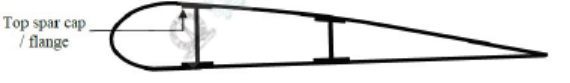
\includegraphics[width=0.5\columnwidth]{figs/21.png}
    \caption{}
    \label{fig:placeholder}
\end{figure}
\begin{multicols}{2}
\begin{enumerate}
\item Yielding
\item Buckling
\item Crushing
\item Creep
\end{enumerate}
\end{multicols}

\item A 2-DOF undamped spring-mass system with two masses and two springs has natural frequencies $\omega_1 = 0.79 \ \text{rad/s}$ and $\omega_2 = 1.538 \ \text{rad/s}$. The mode shapes for the system are given by  
\[
\phi_1 = \myvec{0.732 \\ 1}^T \quad \text{and} \quad \phi_2 = \myvec{-2.73 \\ 1}^T
\]  
If the first mass is displaced by 1 cm, the minimum displacement in cms to be given to the second mass to make the system vibrate in first mode alone is \underline{\hspace{2cm}} (in three decimal place).  

\hfill (GATE AE 2017)

\item An aircraft landing gear can be idealized as a single degree of freedom spring-mass-damper system. The desirable damping characteristics of such a system is:  

\hfill (GATE AE 2017)

\begin{multicols}{2}
\begin{enumerate}
\item Under damped
\item Over damped
\item Critically damped
\item Undamped
\end{enumerate}
\end{multicols}

\item A single degree of freedom spring-mass system of natural frequency $5 \ \text{Hz}$ is modified in the following manners:  

Case 1: Viscous damping with damping ratio $\zeta = 0.2$ is introduced in parallel to the spring.  
Case 2: The original undamped spring-mass system is moved to a surface with coefficient of friction, $\mu = 0.01$.  

The ratio of the damped natural frequency for the cases 1 and 2 is given by \underline{\hspace{2cm}} (in three decimal places).  

\hfill (GATE AE 2017)

\item Which of the following statements about the compatibility equations are true:  
P. Strain compatibility equations must be satisfied in the solution of three-dimensional problems in elasticity.  
Q. Six strains are defined in terms of three displacement functions and can have arbitrary values.  
R. Compatibility equations are an expression of the continuity of displacements.  

\hfill (GATE AE 2017)

\begin{enumerate}
\item P and Q
\item Q and R
\item P and R
\item P, Q and R
\end{enumerate}

\item Matrix 
\[
A = \myvec{2 & 0 & 2 \\ 3 & 7 & 2 \\ 5 & 1 & 7}, \quad 
b = \myvec{4 \\ 4 \\ 5}
\]  

are given. If vector $x$ is the solution to the system of equations $A x = b$, which of the following is true for $x$:  

\hfill (GATE AE 2017)

\begin{enumerate}
\item Solution does not exist
\item Infinite solutions exist
\item Unique solution exists
\item Five possible solutions exist
\end{enumerate}
\item Let matrix 
\[
A = \myvec{2 & -6 \\ 0 & 2}.
\]  
Then for any non-trivial vector 
\[
x = \myvec{x_1 \\ x_2},
\]  
which of the following is true for the value of  
\[
K = x^T A x ?
\]  

\hfill (GATE AE 2017)

\begin{multicols}{2}
\begin{enumerate}
\item $K$ is always less than zero
\item $K$ is always greater than zero
\item $K$ is non-negative
\item $K$ can be anything
\end{enumerate}
\end{multicols}

\item Consider the initial value problem:  

\begin{align*}
\frac{d^2 y}{dt^2} + 4 \frac{dy}{dt} + 6y &= f(t), \quad y(0)=2, \quad \left. \frac{dy}{dt}\right|_{t=0} = 1
\end{align*}

If 
\[
Y(s) = \int_0^\infty y(t) e^{-st} dt, \quad F(s) = \int_0^\infty f(t) e^{-st} dt
\]  
are the Laplace transforms of $y(t)$ and $f(t)$ respectively, then $Y(s)$ is given by:  

\hfill (GATE AE 2017)

\begin{enumerate}
\item $\dfrac{F(s)}{s^2+4s+6}$
\item $\dfrac{F(s)+2s+9}{s^2+4s+6}$
\item $\dfrac{F(s)}{-s^2+4s+6}$
\item $\dfrac{F(s)-2s+9}{s^2+4s+6}$
\end{enumerate}

\item Let $u(x,t)$ denote the displacement of a point on a rod. The displacement satisfies the following equation of motion:  

\begin{align*}
\frac{\partial^2 u}{\partial t^2} - 25 \frac{\partial^2 u}{\partial x^2} &= 0, \quad 0 < x < 1
\end{align*}

with  
\[
u(x,0) = 0.01 \sin(10 \pi x), \quad \frac{\partial u}{\partial t}(x,0)=0; \quad u(0,t)=0, \ u(1,t)=0.
\]  

The value of $u(0.25,1)$ is \underline{\hspace{2cm}} (in three decimal places).  

\hfill (GATE AE 2017)

\item The equation 
\begin{align*}
x^2 \frac{d^2 y}{dx^2} + 5x \frac{dy}{dx} + 4y = 0
\end{align*}
has a solution $y(x)$ that is:  
\hfill (GATE AE 2017)

\begin{enumerate}
\begin{multicols}{2}
\item A polynomial in $x$
\item Finite series in terms of non-integer fractional powers of $x$
\item Consists of negative integer powers of $x$ and logarithmic function of $x$
\item Consists of exponential functions of $x$
\end{multicols}
\end{enumerate}

\item Consider a straight wing with rectangular planform of aspect ratio 10 and with a NACA 0012 airfoil.  
The span effectiveness factor for this wing is 0.95. Assume the flow to be incompressible and governed by thin airfoil theory.  
The lift coefficient of this wing, at an angle of attack of 6 deg, is \underline{\hspace{2cm}} (in three decimal places).  
\hfill (GATE AE 2017)

\item Consider an incompressible flow over a flat plate with the following approximation to the velocity profile:  

\[
\frac{u(y)}{U} = 
\begin{cases} 
\frac{y}{\delta}, & y \leq \delta \\
1, & y > \delta
\end{cases}
\]

where $\delta$ is the boundary layer thickness and $U$ the free-stream speed.  
The normalized momentum thickness $(\theta / \delta)$ for this profile is \underline{\hspace{2cm}} (in three decimal places).  
\hfill (GATE AE 2017)

\item An idealized velocity field is given by  
\[
\vec{V} = 4tx \hat{i} - 2t^2 y \hat{j} + 4xz \hat{k}.
\]  

At point $(-1,1,0)$ and at $t=1$, the magnitude of the material acceleration vector of the fluid element is \underline{\hspace{2cm}}.  
\hfill (GATE AE 2017)

\item A trace from the schlieren photograph of the flow around a corner reveals the edges of the expansion fan as shown below.  
The leading and trailing edges of the expansion fan make the angles as shown.  
Assuming $\gamma = 1.4$, the angle of the expansion fan (in degrees) is \underline{\hspace{2cm}} (in two decimal places).  

Prandtl Meyer function is given by  
\begin{align*}
\nu(M) = \sqrt{\frac{\gamma+1}{\gamma-1}} \, \tan^{-1} \left( \sqrt{\frac{\gamma-1}{\gamma+1}(M^2-1)} \right) - \tan^{-1}\left(\sqrt{M^2-1}\right)
\end{align*}  
\begin{figure}[H]
    \centering
    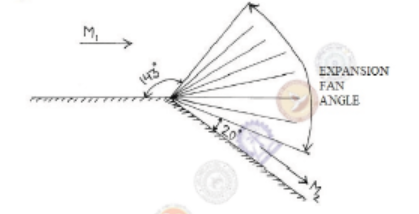
\includegraphics[width=0.5\columnwidth]{figs/34.png}
    \caption{}
    \label{fig:placeholder}
\end{figure}
\hfill (GATE AE 2017)  

\item A strong normal shock wave, with a pressure ratio of 29 across it, is travelling into stationary air $(\gamma=1.4)$ at $T=280 \,K$ in a straight duct (see figure).  
The magnitude of the velocity of the air induced behind the shock wave is \underline{\hspace{2cm}} m/s. (round off to nearest integer).  

(Gas constant = 287 J/kg·K; Shock wave relations:  

\begin{align*}
\frac{p_2}{p_1} &= 1 + \frac{2\gamma}{\gamma+1}(M^2-1) \\
\frac{\rho_2}{\rho_1} &= \frac{(\gamma+1)M^2}{(\gamma-1)M^2+2}
\end{align*}  
\begin{figure}[H]
    \centering
    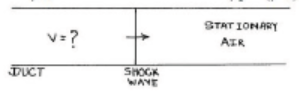
\includegraphics[width=0.5\columnwidth]{figs/35.png}
    \caption{}
    \label{fig:placeholder}
\end{figure}
\hfill (GATE AE 2017)  

\item In the figure below, water exits from a nozzle into atmospheric pressure of 101 kPa. If the exit velocity is $V_2 = 8 \, \text{m/s}$ and friction is neglected, the magnitude of the axial force on the flange at location 1 required to keep the nozzle attached to the pipe is \underline{\hspace{2cm}} N (round to nearest integer).  

\hfill (GATE AE 2017)  
\begin{figure}[H]
    \centering
    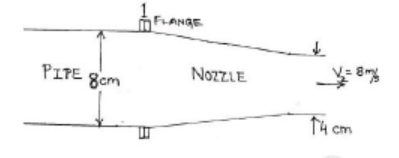
\includegraphics[width=0.5\columnwidth]{figs/36.png}
    \caption{}
    \label{fig:placeholder}
\end{figure}
\item A football, meant to be thrown at 100 km/h in sea level air $(\rho = 1.22 \, \text{kg/m}^3, \mu = 1.78 \times 10^{-5} \, \text{N·s/m}^2)$, is to be tested using a one-quarter scale model in a water tunnel $(\rho = 1000 \, \text{kg/m}^3, \mu = 10^{-3} \, \text{N·s/m}^2)$.  
For dynamic similarity, the ratio of the model force to the prototype force is \underline{\hspace{2cm}} (round to nearest integer).  

\hfill (GATE AE 2017)  

\item An aircraft model was tested in a low speed wind-tunnel (Reynolds number $= 2 \times 10^6$ based on wing mean chord). The variation of pitching moment coefficient $(C_m)$ with angle of attack $(\alpha)$ for two elevator deflections $(\delta_e)$ as recorded during this test is presented below.  

Based on the result presented in the figure above, the value of elevator control power $(C_{m\delta_e})$ in per radian will be \underline{\hspace{2cm}} (in three decimal place).  

\hfill (GATE AE 2017)  
\begin{figure}[H]
    \centering
    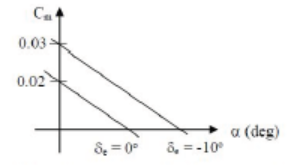
\includegraphics[width=0.5\columnwidth]{figs/38.png}
    \caption{}
    \label{fig:placeholder}
\end{figure}

\item A pilot was flying a single engine propeller aircraft and maintaining a steady level flight at a lift coefficient, $C_L = 0.5$ at an altitude of 500 m. Due to some emergency, at the same altitude (500 m), the pilot had to fully deploy the landing gear. If the pilot wants to maintain steady level flight at the same $C_L = 0.5$ and at the same altitude, which of the following control actions should the pilot undertake:  

\hfill (GATE AE 2017)  

\begin{enumerate}
\item move the elevator up, and decrease the throttle  
\item move the elevator up, and increase the throttle  
\item move the elevator down, and decrease the throttle  
\item move the elevator down, and increase the throttle  
\end{enumerate}

\item A conventional low speed aircraft had the following aerodynamic characteristics: $C_{D0} = 0.020, \ \epsilon = 1.0$ (Oswald efficiency).  
The aircraft was flown to maintain a steady level flight and for minimum thrust required, at a lift coefficient of $C_L = 0.8$. The numerical value of the aspect ratio of the wing is \underline{\hspace{2cm}} (in three decimal places).  

\hfill (GATE AE 2017)  

\item A batch of aluminium alloy yields in uniaxial tension at the stress of 330 MN/m$^2$. If this material is subjected to the following state of stress: $\sigma_x = 140$ MN/m$^2$, $\sigma_y = -70$ MN/m$^2$, $\sigma_z = 0$, $\tau_{xy} = x$ MN/m$^2$, $\tau_{yz} = 0$, and $\tau_{zx} = 0$. The value of $x$ that would result in yielding according to the Von Mises failure criterion is \underline{\hspace{2cm}} (in three decimal places).  

\hfill (GATE AE 2017)  

\item The roots obtained by solving longitudinal characteristic equations of motion for a statically stable aircraft are given below:  

\[
\lambda_{1,2} = -0.02 \pm 0.30i, \quad \lambda_{3,4} = -2.00 \pm 2.50i, \quad \text{where } i = \sqrt{-1}
\]

The undamped short-period longitudinal natural frequency (radians/sec) and damping ratio, in that order, are close to  

\hfill (GATE AE 2017)  

\begin{enumerate}
\item 3.40, 0.73  
\item 3.36, 0.65  
\item 3.83, 0.56  
\item 3.20, 0.63  
\end{enumerate}
\item An aircraft is to be designed to ensure that it has enough excess power to achieve steady climb at flight path angle, $\gamma = 10$ degrees, maintaining $\dfrac{C_L}{C_D} = 10.0$. The numerical value of the thrust to weight ratio of the complete aircraft to meet the above requirement under standard atmospheric condition will be \underline{\hspace{2cm}} (in three decimal places).  

\hfill (GATE AE 2017)  

\item A conventional aircraft was analyzed to estimate the contribution of wing towards $C_{m0}$ (Cm at $\alpha = 0$) of the whole aircraft. The wing was installed with zero setting angle along the fuselage reference line. Further, the wing was laid such that $X_{\alpha,w} = 0.3$, and $X_{ac,aircraft} = 0.4$. $X_{\alpha,w}$ and $X_{ac,aircraft}$ are the non-dimensional distances, from the leading edge of the wing, of the aerodynamic center of the wing and center of gravity of the aircraft respectively. The wing had the following aerodynamic characteristics:  

\[
C_{L0} = 0.20, \quad C_{mac,wing} = -0.02
\]

The numerical value of $C_{m0,w}$ (contribution of the wing to $C_{m0}$) about the CG of the aircraft is \underline{\hspace{2cm}} (in two decimal places).  

\hfill (GATE AE 2017)  

\item In a combustor, gaseous Octane ($C_8H_{18}$) and air are to be burned in stoichiometric proportions. If the required flowrate of air is 1 kg/s, what should be the corresponding flow rate of Octane?  

\hfill (GATE AE 2017)  

\begin{enumerate}
\item 0.066 kg/s  
\item 15.15 kg/s  
\item 0.16 kg/s  
\item 6.25 kg/s  
\end{enumerate}
\item The given diagram represents the velocity triangles at the leading edge (1) and trailing edge (2) at the mean radius of a single stage axial compressor rotor. The stage efficiency of the compressor is 0.8. The stagnation temperature of air entering the stage is 298 K and the specific heat at constant pressure for air is 1.005 kJ/kgK. The ratio of specific heats for air is 1.4. Considering actual work in the rotor is equal to the ideal work, the pressure ratio for the stage is equal to \underline{\hspace{2cm}} (in two decimal points).  
\begin{figure}[H]
    \centering
    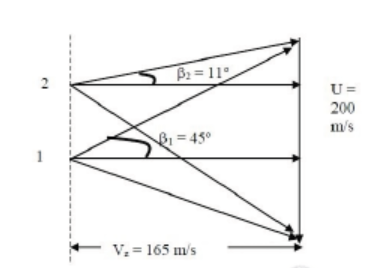
\includegraphics[width=0.5\columnwidth]{figs/46.png}
    \caption{}
    \label{fig:placeholder}
\end{figure}

\hfill (GATE AE 2017)  

\item An aircraft with a turbojet engine, having an inlet area of 1 m$^2$, is flying at 270 m/s at an altitude where the atmospheric pressure is equal to 0.9 bar and the ambient temperature is equal to 290 K. The stagnation pressure and temperature at the exit of the turbine are equal to 1.6 bar and 774 K respectively. The specific heat at constant pressure of the burned gases is equal to 1.147 kJ/kgK and the ratio of specific heats is equal to 1.33. Considering ideal expansion in the nozzle with no losses, the specific thrust produced by the engine is \underline{\hspace{2cm}} Ns/kg (in one decimal place).  

\hfill (GATE AE 2017)  

\item Air, at 450 K stagnation temperature and at a rate of 50 kg/s, enters the combustor of a turbofan engine and is burned with 1 kg/s of Aviation Kerosene (Heating value 44 MJ/kg). The specific heat at constant pressure for the incoming air and the burned products are 1.005 kJ/kgK and 1.147 kJ/kgK respectively. Considering 100\% burner efficiency, the stagnation temperature at the exit of the combustor is equal to \underline{\hspace{2cm}} K (in one decimal place).  

\hfill (GATE AE 2017)  
\item A single stage chemical rocket, having an initial mass of 10,000 kg and specific impulse of 450 s, is launched from the surface of the earth and has to reach the escape velocity (11 km/s) at burn out. Consider $g_e = 9.8$ m/s$^2$. If the atmospheric drag and the effect of gravity are to be neglected, the mass of propellant to be carried by the rocket is equal to \underline{\hspace{2cm}} kg (in one decimal place).  

\hfill (GATE AE 2017)  

\item A centrifugal compressor requires 1800 kW of power to compress 10 kg/s of air. Consider the whirl velocity component is equal to the impeller speed (i.e., no slip) and no losses in the impeller. If the impeller has to rotate at 1900 rad/s, the diameter of the impeller is to be \underline{\hspace{2cm}} m (in two decimal places).  

\hfill (GATE AE 2017)  

\item An aircraft wing is idealized as a cantilever beam of constant width and length $l$ with a tip mass of weight $W$ (Newtons) and has a uniformly distributed loading of $q_0$ (Newtons/m) as shown in the figure. Flexural rigidity = $EI$ and $q_0 l = 10W$.  
\begin{figure}[H]
    \centering
    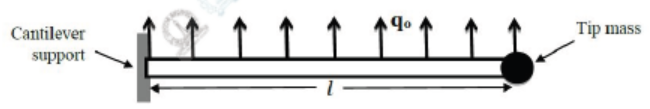
\includegraphics[width=0.5\columnwidth]{figs/51.png}
    \caption{}
    \label{fig:placeholder}
\end{figure}
The upward deflection of the tip of the aircraft wing under the given loading can be expressed as:  

\begin{align*}
\delta &= k \frac{W l^3}{EI}
\end{align*}  

The value of $k$ is \underline{\hspace{2cm}} (in three decimal places).  

\hfill (GATE AE 2017)  
\item For the state of plane stress shown in the figure, the minimum principal stress is $-7$ MN/m$^2$. The normal stress $\sigma_x$ in MN/m$^2$ is equal to \underline{\hspace{2cm}} (round to nearest integer).  

\hfill (GATE AE 2017)  

\begin{figure}[H]
    \centering
    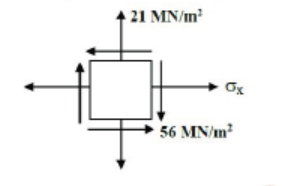
\includegraphics[width=0.5\columnwidth]{figs/52.png}
    \caption{}
    \label{fig:placeholder}
\end{figure}
\item The maximum normal stress in MN/m$^2$ for the thin walled beam of square cross section of outer dimension 120 mm $\times$ 120 mm and wall thickness 1 mm under the action of moment $M_z = 96$ Nm as shown in the figure is \underline{\hspace{2cm}} (in three decimal places).  

\hfill (GATE AE 2017)  

\begin{figure}[H]
    \centering
    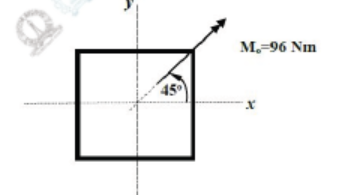
\includegraphics[width=0.5\columnwidth]{figs/53.png}
    \caption{}
    \label{fig:placeholder}
\end{figure}

\item The idealized cross section of a thin-walled wing box structure shown in the figure is subjected to an anticlockwise torque of 10 kNm. The corresponding shear-flow distribution under this loading condition is shown in the figure. The area of each cell is $A_1 = 300 \times 10^3$ mm$^2$ and $A_2 = 250 \times 10^3$ mm$^2$. The ratio of the unknowns $\tfrac{x}{y}$ is given by \underline{\hspace{2cm}} (in three decimal places).  

\hfill (GATE AE 2017)  

\begin{figure}[H]
    \centering
    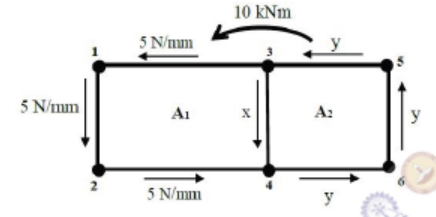
\includegraphics[width=0.5\columnwidth]{figs/54.png}
    \caption{}
    \label{fig:placeholder}
\end{figure}

\item The natural frequency of the system suspended by two identical springs of stiffness $k$ as shown in the figure is given by $\omega_n = a \sqrt{\tfrac{k}{m}}$ for small displacement. Both the springs make an angle of $45^\circ$ with the horizontal. The value of $a$ is \underline{\hspace{2cm}} (in two decimal places).  

\hfill (GATE AE 2017)  

\begin{figure}[H]
    \centering
    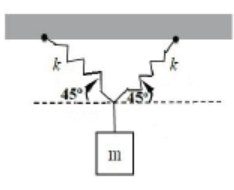
\includegraphics[width=0.5\columnwidth]{figs/55.png}
    \caption{}
    \label{fig:placeholder}
\end{figure}

\item The ninth and the tenth of this month are Monday and Tuesday \underline{\hspace{2cm}}.  

\hfill (GATE AE 2017) 
\begin{enumerate}
\item figuratively  
\item retrospectively  
\item respectively  
\item rightfully  
\end{enumerate}  

 

\item It is \underline{\hspace{2cm}} to read this year's textbook \underline{\hspace{2cm}} the last year's.  

\hfill (GATE AE 2017)  
\begin{enumerate}
\item easier, than  
\item most easy, than  
\item easier, from  
\item easiest, from  
\end{enumerate}  


\item A rule states that in order to drink beer, one must be over 18 years old. In a bar, there are 4 people.  
P is 16 years old, Q is 25 years old, R is drinking milkshake and S is drinking a beer.  
What must be checked to ensure that the rule is being followed? 

\hfill (GATE AE 2017)  

\begin{enumerate}
\item Only P's drink  
\item Only P's drink and S's age  
\item Only S's age  
\item Only P's drink, Q's drink and S's age  
\end{enumerate}  

\item Fatima starts from point P, goes North for 3 km, and then East for 4 km to reach point Q.  
She then turns to face point P and goes 15 km in that direction. She then goes North for 6 km.  
How far is she from point P, and in which direction should she go to reach point P?  

\hfill (GATE AE 2017)  
\begin{enumerate}
\item 8 km, East  
\item 12 km, North  
\item 6 km, East  
\item 10 km, North  
\end{enumerate}  

\item 500 students are taking one or more courses out of Chemistry, Physics, and Mathematics. Registration records indicate course enrolment as follows: Chemistry (329), Physics (186), Mathematics (295), Chemistry and Physics (83), Chemistry and Mathematics (217), and Physics and Mathematics (63). How many students are taking all 3 subjects?  

\hfill (GATE AE 2017)

\begin{enumerate}
\begin{multicols}{4}
\item 37
\item 43
\item 47
\item 53
\end{multicols}
\end{enumerate}

\item "If you are looking for a history of India, or for an account of the rise and fall of the British Raj, or for the reason of the cleaving of the subcontinent into two mutually antagonistic parts and the effects this mutilation will have in the respective sections, and ultimately on Asia, you will not find it in these pages; for though I have spent a lifetime in the country, I lived too near the seat of events, and was too intimately associated with the actors, to get the perspective needed for the impartial recording of these matters."  
Which of the following statements best reflects the author's opinion?

\hfill (GATE AE 2017)

\begin{enumerate}
\item An intimate association does not allow for the necessary perspective.
\item Matters are recorded with an impartial perspective.
\item An intimate association offers an impartial perspective.
\item Actors are typically associated with the impartial recording of matters.
\end{enumerate}

\item Each of P, Q, R, S, W, X, Y and Z has been married at most once. X and Y are married and have two children P and Q. Z is the grandfather of the daughter S of P. Further, Z and W are married and are parents of R. Which one of the following must necessarily be FALSE?

\hfill (GATE AE 2017)

\begin{enumerate}
\item X is the mother-in-law of R
\item P and R are not married to each other
\item P is a son of X and Y
\item Q cannot be married to R
\end{enumerate}

\item 1200 men and 500 women can build a bridge in 2 weeks. 900 men and 250 women will take 3 weeks to build the same bridge. How many men will be needed to build the bridge in one week?

\hfill (GATE AE 2017)

\begin{enumerate}
\begin{multicols}{4}
\item 3000
\item 3300
\item 3600
\item 3900
\end{multicols}
\end{enumerate}

\item The number of 3-digit numbers such that the digit 1 is never to the immediate right of 2 is \underline{\hspace{2cm}}.

\hfill (GATE AE 2017)

\begin{enumerate}
\begin{multicols}{4}
\item 781
\item 791
\item 881
\item 891
\end{multicols}
\end{enumerate}

\item A contour line joins locations having the same height above the mean sea level. The following is a contour plot of a geographical region. Contour lines are shown at 25 m intervals in this plot. Which of the following is the steepest path leaving from P?

\begin{figure}[H]
    \centering
    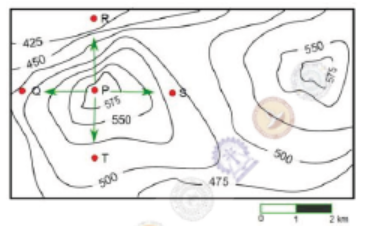
\includegraphics[width=0.5\columnwidth]{figs/65.png}
    \caption{}
    \label{fig:placeholder}
\end{figure}

\hfill (GATE AE 2017)

\begin{enumerate}
\begin{multicols}{4}
\item P to Q
\item P to R
\item P to S
\item P to T
\end{multicols}
\end{enumerate}


\end{enumerate}

\end{flushleft}
\end{document}

